\documentclass[a4paper,12pt]{article} % The document class with options

\usepackage[T1]{fontenc}
\usepackage{enumitem}
\usepackage{amsmath}
\usepackage{amsfonts}
\usepackage{microtype}
\usepackage{graphicx}
\usepackage{epstopdf}
% chktex-file 1
% chktex-file 3
% chktex-file 18
% chktex-file 24
% chktex-file 25

\begin{document}
%\setlength{\parskip}{1em} 
%\setlength{\parindent}{0pt}
\newcommand{\vect}[1]{\mathbf{#1}}

\title{MECH 503 Homework 1}
\author{Jincong Li \\ 60539939}
\date{Jan 26th}
\maketitle

\section{\textbf{Question 1}}

\begin{enumerate}[label= (\alph*)]
    \item \[ \nu_i u_i = \sum_{i=1}^{n} \nu_i u_i \]
    
    \item \[ \delta_{ii} = \sum_{i=1}^{n} \delta_{ii} = n \]

    \item \[ \nu_{i,i} = \sum_{i=1}^{n} \frac{\partial \nu_i}{\partial x_i} \]

    \item \[ \delta_{ij,j} = \sum_{j=1}^{n} \frac{\partial \delta_{ij}}{\partial x_j}\]

    \item \[ \epsilon_{ijk} v_j u_k = \sum_{j=1}^{n} \sum_{k=1}^{n} \epsilon_{ijk} v_j u_k \]

    \item \[ \delta_{mi} \delta_{mj} T_{ij} = \sum_{i=1}^{n} \sum_{j=1}^{n} \delta_{mi} \delta_{mj} T_{ij} = T_{mm} \]

    \item \[ Q_{ij} T_{ik} Q_{km} = \sum_{j=1}^{n} \sum_{k=1}^{n} Q_{ij} T_{ik} Q_{km} \]

    \item \[ \epsilon_{ijk} \sigma_{jk} = \sum_{j=1}^{n} \sum_{k=1}^{n} \epsilon_{ijk} \sigma_{jk} \]
\end{enumerate}

\section{\textbf{Question 2}}

\begin{enumerate}[label= (\alph*)]
    \item \[ (u \times v) \cdot w = \varepsilon_{ijk} u_j v_k w_i \]

    \item \[ \text{det } T = \varepsilon_{ijk} T_{1i} T_{2j} T_{3k} \]
    
    \item \[ (\nabla \times v)_i = \varepsilon_{ijk} \partial_j v_k \]
    
    \item \[ \nabla \cdot v = \partial_i v_i \]
    
    \item \[ (\nabla \times T)_{ij} = \varepsilon_{jkl} \partial_k T_{il} \]
    
    \item \[ (\nabla \times (\nabla T))_i = \varepsilon_{ijk} \partial_j (\partial_k T) \]
    
    \item \[ (\nabla \cdot T)_i = \partial_j T_{ij} \]
\end{enumerate}

\newpage
\section{\textbf{Question 3}}
\begin{align*}
    \intertext{Define a second order tensor $C$ such that}
    \vect{C} &= \vect{A} \cdot \vect{B}\\
    \Longleftrightarrow C_{ij} &= A_{ik} \cdot B_{kj}\\
    \text{det \textbf{C}} &= \epsilon _{ijk} C_{1i} C_{2j} C_{3k}\\
    &= \epsilon _{ijk} (A_{1l} B_{li}) (A_{2m} B_{mj}) (A_{3n} B_{nk})\\
    &= \epsilon _{ijk} (A_{1l} A_{2m} A_{3n}) (B_{li} B_{mj}  B_{nk})\\
    \intertext{Now consider the determinant of $A$ and $B$ separately}
    \text{det \textbf{A}} &= \epsilon _{lmn} A_{1l} A_{2m} A_{3n}\\
    \text{det \textbf{B}} &= \epsilon _{ijk} B_{li} B_{mj} B_{nk}\\
    \text{det \textbf{A}} \cdot \text{det \textbf{B}} &=(\epsilon _{lmn} A_{1l} A_{2m} A_{3n})(\epsilon _{ijk} B_{li} B_{mj} B_{nk})
    \intertext{Thus, one can conclude the following}
    \text{det (\textbf{A $\cdot$ B})} &= \text{det \textbf{A}} \cdot \text{det \textbf{B}}
\end{align*}

\newpage
\section{\textbf{Question 4}}
\begin{align*}
    Q_{ij} Q^{-1}_{jk} &= Q_{ij} Q^T_{kj} = \delta_{ik} \\
    \implies Q^{-1}_{jk} &= Q^T_{kj}\\
    (QQ^T)_{ij} &= Q_{ik} Q^T_{kj} \\
&= Q_{ik} Q_{jk} \\
&= \delta_{ij} \\
\implies QQ^T &= I\\
(Q^TQ)_{ij} &= Q^T_{ik} Q_{kj} \\
&= Q_{ki} Q_{kj} \\
&= \delta_{ji} \\
&= \delta_{ij} \\
\implies Q^TQ &= I
\end{align*}

\newpage
\section{\textbf{Question 5}}
\begin{figure}[htbp]
    % \centering
    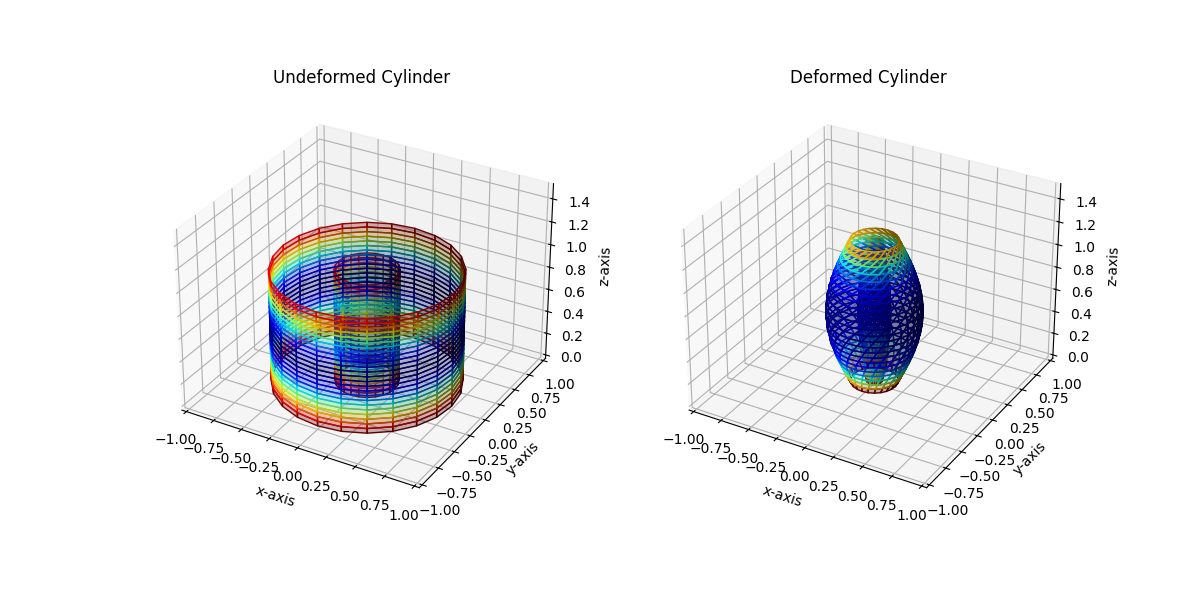
\includegraphics[scale=0.5]{MECH503HW1Q5.png}
    
    \caption{Undeformed and Deformed Cylinder Visualization}
\label{figure}
\end{figure}

\end{document}